\documentclass[11pt,a4paper]{article}

% Packages
\usepackage[utf-8]{inputenc}
\usepackage[margin=1in]{geometry}
\usepackage{xcolor}
\usepackage{listings}
\usepackage{hyperref}
\usepackage{enumitem}
\usepackage{graphicx}
\usepackage{tikz}
\usetikzlibrary{positioning,shapes,arrows}

% Code listing configuration
\definecolor{codegray}{rgb}{0.5,0.5,0.5}
\definecolor{codepurple}{rgb}{0.58,0,0.82}
\definecolor{backcolour}{rgb}{0.95,0.95,0.92}

\lstdefinestyle{mystyle}{
    backgroundcolor=\color{backcolour},
    commentstyle=\color{codegray},
    keywordstyle=\color{blue},
    numberstyle=\tiny\color{codegray},
    stringstyle=\color{codepurple},
    basicstyle=\ttfamily\footnotesize,
    breakatwhitespace=false,
    breaklines=true,
    captionpos=b,
    keepspaces=true,
    numbers=left,
    numbersep=5pt,
    showspaces=false,
    showstringspaces=false,
    showtabs=false,
    tabsize=2
}

\lstset{style=mystyle}

% Hyperlink setup
\hypersetup{
    colorlinks=true,
    linkcolor=blue,
    urlcolor=blue,
}

% Title
\title{\textbf{Demystifying Data Engineering:\\Lessons from Building a Web Scraper}}
\author{Learning Synthesis from SEP Data Scraper Project}
\date{October 30, 2025}

\begin{document}

\maketitle

\begin{abstract}
This document captures fundamental data engineering insights discovered organically while building a web scraper for Mexican education statistics. Rather than learning from textbooks or consultants, we encountered core architectural patterns and design decisions through practical necessity. The result: a clear mental framework for understanding data systems that cuts through industry jargon and reveals the essential trade-offs underlying most data engineering work.
\end{abstract}

\section{Learning Objectives}

By the end of this document, you should be able to:

\begin{enumerate}
    \item \textbf{Identify the three fundamental axes} that govern data engineering architecture decisions
    \item \textbf{Recognize common patterns} (like medallion architecture) when they emerge naturally in your work
    \item \textbf{Make informed trade-offs} between competing approaches based on your specific constraints
    \item \textbf{Translate buzzword-heavy concepts} into simple, actionable design principles
    \item \textbf{Design crash-resistant systems} that preserve work incrementally rather than losing progress
\end{enumerate}

\section{Context: The Problem}

\subsection{Project Requirements}

The task was to scrape education statistics from Mexico's SEP (Secretaría de Educación Pública) database:

\begin{itemize}
    \item \textbf{Scope}: 32 states, each containing multiple municipios (municipalities)
    \item \textbf{Data depth}: Individual municipio-level statistics requiring navigation through nested pages
    \item \textbf{Output}: Structured data suitable for analysis in R
    \item \textbf{Constraints}: Single machine, no cloud infrastructure, exploratory project with uncertain final format
\end{itemize}

\subsection{Initial Approach}

The first iteration was straightforward: sequential scraping that processed one state at a time, collecting data in memory and writing batch files. This worked but revealed problems:

\begin{itemize}
    \item \textbf{Speed}: Too slow for 32 states with dozens of municipios each
    \item \textbf{Disk space}: JSON files accumulating rapidly
    \item \textbf{Fragility}: Browser crashes meant losing all progress since last state completion
    \item \textbf{Uncertainty}: Unclear what final data structure should look like
\end{itemize}

These constraints forced us to confront fundamental architectural questions.

\section{The Accidental Architecture: Medallion Pattern}

\subsection{What We Built Without Knowing It}

While deciding how to handle raw data versus cleaned data, we naturally arrived at a three-layer structure:

\begin{enumerate}
    \item \textbf{Raw Layer (``Bronze'')}: JSON files containing everything scraped
    \begin{itemize}
        \item All fields captured, including potentially irrelevant data
        \item Messy structure mirroring website's HTML organization
        \item Nothing filtered or validated
    \end{itemize}

    \item \textbf{Staging Layer (``Silver'')}: CSV converter that cleans and structures
    \begin{itemize}
        \item Extracts relevant fields
        \item Normalizes formats and handles missing values
        \item Validates data integrity
    \end{itemize}

    \item \textbf{Production Layer (``Gold'')}: Analysis-ready datasets
    \begin{itemize}
        \item Optimized for R analysis workflows
        \item Aggregated or joined as needed
        \item Documentation and metadata included
    \end{itemize}
\end{enumerate}

\subsection{The Revelation}

This pattern has a name in industry: \textit{medallion architecture} (also called bronze/silver/gold layers). But we didn't need to know that to arrive at it. The pattern emerged from a simple principle:

\begin{quote}
\textbf{Capture everything first, clean later.} Disk space is cheap; re-scraping is expensive.
\end{quote}

\subsection{Why This Matters}

The key learning isn't that medallion architecture is some brilliant framework. It's that \textbf{sensible patterns emerge naturally from understanding your constraints}. You don't need an expensive consultant to tell you not to throw away raw data.

\begin{lstlisting}[language=bash,caption={Our emergent directory structure}]
/data
  /raw              # Bronze: JSON as scraped
    aguascalientes.json
    baja-california.json
    ...
  /processed        # Silver: Cleaned CSVs
    municipios.csv
    estados.csv
  /analysis         # Gold: R-ready datasets
    enrollment-trends.csv
    regional-comparison.csv
\end{lstlisting}

\section{The Three Core Decisions Framework}

Through iteration and problem-solving, we discovered that almost every data engineering decision reduces to three fundamental axes. Understanding these axes provides more insight than memorizing framework names.

\subsection{Axis 1: Centralized vs. Distributed}

\textbf{The Question}: Are you processing on one machine or coordinating across multiple machines?

\begin{itemize}
    \item \textbf{Centralized}: All work happens on a single machine
    \begin{itemize}
        \item Limited by that machine's CPU, memory, and disk
        \item Simple: no network coordination, no data synchronization issues
        \item Examples: Your laptop, a single server, one database instance
    \end{itemize}

    \item \textbf{Distributed}: Work is coordinated across multiple machines
    \begin{itemize}
        \item Can scale beyond single-machine limits
        \item Complex: network failures, data consistency, coordination overhead
        \item Examples: Hadoop clusters, distributed databases, microservices
    \end{itemize}
\end{itemize}

\textbf{Our Choice}: Centralized. We had one laptop and no need for multi-machine scale.

\textbf{Key Insight}: Most projects don't need distributed systems. Single machines are incredibly powerful in 2025. Don't reach for distributed solutions until you've exhausted centralized optimizations.

\subsection{Axis 2: Sequential vs. Parallel}

\textbf{The Question}: Are you doing one task at a time or multiple tasks simultaneously \textit{on the same machine}?

\begin{itemize}
    \item \textbf{Sequential}: Process items one by one
    \begin{itemize}
        \item Simple to reason about: no race conditions, predictable order
        \item Underutilizes modern multi-core processors
        \item Examples: Looping through a list with single thread
    \end{itemize}

    \item \textbf{Parallel}: Process multiple items at once on one machine
    \begin{itemize}
        \item Uses multiple CPU cores or I/O concurrency
        \item Faster for I/O-bound (network, disk) or CPU-bound tasks
        \item Requires coordination: thread safety, resource limits
        \item Examples: Thread pools, async/await patterns, worker processes
    \end{itemize}
\end{itemize}

\textbf{Critical Distinction}: Parallel $\neq$ Distributed. Parallel means multiple tasks on \textit{one} machine. You can have:
\begin{itemize}
    \item Centralized + Sequential (slowest, simplest)
    \item Centralized + Parallel (our choice)
    \item Distributed + Sequential (rare, usually doesn't make sense)
    \item Distributed + Parallel (complex, maximum throughput)
\end{itemize}

\textbf{Our Choice}: Parallel. We ran 3-5 browser contexts simultaneously. Our bottleneck was network I/O (waiting for page loads), not CPU, so parallelism provided massive speedup without complexity of distributed systems.

\begin{lstlisting}[language=JavaScript,caption={Parallel scraping with browser contexts}]
// Sequential: Slow but simple
for (const state of states) {
    await scrapeState(state);
}

// Parallel: Fast for I/O-bound work
const promises = states.map(state => scrapeState(state));
await Promise.all(promises);

// Controlled parallel: Best of both worlds
const limit = 5; // 5 concurrent scrapers
for (let i = 0; i < states.length; i += limit) {
    const batch = states.slice(i, i + limit);
    await Promise.all(batch.map(state => scrapeState(state)));
}
\end{lstlisting}

\subsection{Axis 3: Batch vs. Stream}

\textbf{The Question}: Do you load all data into memory, process it, then write? Or process and write incrementally?

\begin{itemize}
    \item \textbf{Batch}: Load → Process → Write
    \begin{itemize}
        \item All data in memory at once
        \item Can see entire dataset: enables operations requiring full context
        \item Memory-limited: crashes if dataset exceeds RAM
        \item Examples: Reading entire CSV into Pandas DataFrame, ``SELECT *'' queries
    \end{itemize}

    \item \textbf{Stream}: Process and write item-by-item
    \begin{itemize}
        \item Constant memory usage regardless of dataset size
        \item Can't see full dataset: limited to operations on current item
        \item Crash-resistant: work is saved incrementally
        \item Examples: Processing log files line-by-line, SAX XML parsers
    \end{itemize}
\end{itemize}

\textbf{Our Evolution}: Started with batch per state (load all municipios, write state file). Evolved to streaming (write each municipio immediately).

\textbf{Key Insight}: Streaming isn't primarily about speed—it's about \textit{memory management} and \textit{crash resistance}. Writing incrementally means a crash at municipio 47 doesn't lose municipios 1-46.

\begin{lstlisting}[language=JavaScript,caption={Batch vs Stream scraping}]
// Batch approach (original)
async function scrapeState(state) {
    const municipios = [];
    for (const muni of state.municipios) {
        const data = await scrapeMunicipio(muni);
        municipios.push(data); // Accumulate in memory
    }
    // Write everything at end
    await fs.writeFile(`${state.name}.json`,
                       JSON.stringify(municipios));
}

// Stream approach (improved)
async function scrapeState(state) {
    const fileStream = fs.createWriteStream(`${state.name}.json`);
    fileStream.write('['); // Start JSON array

    for (const muni of state.municipios) {
        const data = await scrapeMunicipio(muni);
        fileStream.write(JSON.stringify(data) + ',');
        // Written immediately - crash safe!
    }

    fileStream.write(']');
    fileStream.end();
}
\end{lstlisting}

\subsection{The Complete Framework}

Every data system can be characterized by these three decisions:

\begin{center}
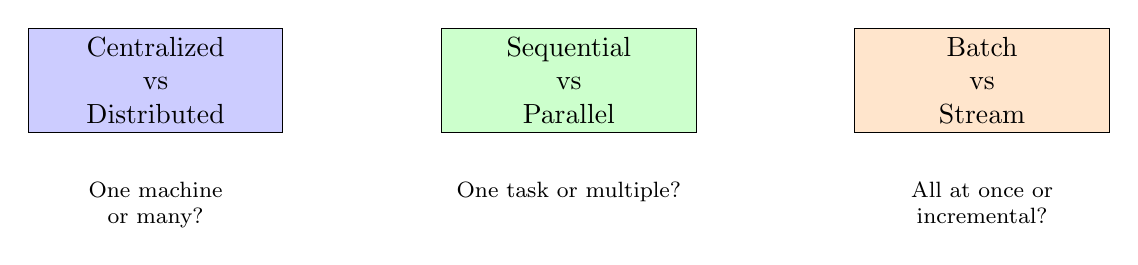
\begin{tikzpicture}[node distance=2cm]
    \node[rectangle, draw, fill=blue!20, text width=3cm, align=center] (c) {Centralized\\vs\\Distributed};
    \node[rectangle, draw, fill=green!20, text width=3cm, align=center, right=of c] (s) {Sequential\\vs\\Parallel};
    \node[rectangle, draw, fill=orange!20, text width=3cm, align=center, right=of s] (b) {Batch\\vs\\Stream};

    \node[below=0.5cm of c, text width=3cm, align=center, font=\footnotesize] {One machine or many?};
    \node[below=0.5cm of s, text width=3cm, align=center, font=\footnotesize] {One task or multiple?};
    \node[below=0.5cm of b, text width=3cm, align=center, font=\footnotesize] {All at once or incremental?};
\end{tikzpicture}
\end{center}

\textbf{Our final architecture}: Centralized + Parallel + Stream

This gave us speed (parallel), crash resistance (stream), and simplicity (centralized).

\section{Practical Application: Scraper Evolution}

\subsection{Version 1: The Naive Approach}

\textbf{Architecture}: Centralized + Sequential + Batch

\begin{lstlisting}[language=JavaScript,caption={First iteration}]
// Process states one by one
for (const state of states) {
    const municipios = [];

    // Sequential municipio scraping
    for (const muni of state.municipios) {
        const data = await scrapeMunicipio(muni);
        municipios.push(data);
    }

    // Batch write at end
    await fs.writeFile(`${state.name}.json`,
                       JSON.stringify(municipios));
}
\end{lstlisting}

\textbf{Problems Encountered}:
\begin{itemize}
    \item Estimated completion time: 8+ hours for all states
    \item Browser crashed at state 15: lost all progress
    \item Disk filled up with 32 large JSON files
    \item No visibility into progress within each state
\end{itemize}

\subsection{Version 2: Parallel + Stream}

\textbf{Architecture}: Centralized + Parallel + Stream

\begin{lstlisting}[language=JavaScript,caption={Improved version}]
// Process 5 states concurrently
const CONCURRENT_STATES = 5;

async function scrapeWithStreaming(state) {
    const stream = fs.createWriteStream(
        `./data/raw/${state.name}.json`
    );

    stream.write('{"municipios": [');

    // Within each state, process municipios in parallel too
    const chunks = chunkArray(state.municipios, 3);
    let first = true;

    for (const chunk of chunks) {
        const results = await Promise.all(
            chunk.map(m => scrapeMunicipio(m))
        );

        for (const data of results) {
            if (!first) stream.write(',');
            stream.write(JSON.stringify(data));
            first = false;

            // Crash happens here?
            // All previous municipios are saved!
        }
    }

    stream.write(']}');
    stream.end();
}

// Run multiple states in parallel
for (let i = 0; i < states.length; i += CONCURRENT_STATES) {
    const batch = states.slice(i, i + CONCURRENT_STATES);
    await Promise.all(batch.map(s => scrapeWithStreaming(s)));
}
\end{lstlisting}

\textbf{Improvements}:
\begin{itemize}
    \item Completion time: Under 2 hours (4x speedup)
    \item Crash at municipio 47 only loses current batch of 3 municipios
    \item Can monitor progress by watching file sizes grow
    \item Better resource utilization: network I/O parallelized
\end{itemize}

\section{Design Trade-offs: Raw Data vs. Parsed Data}

\subsection{The Decision Point}

When building the scraper, we faced a choice: should we parse and structure data \textit{during} scraping, or capture everything raw and parse later?

\subsection{Option A: Capture Everything Raw (Our Choice)}

\textbf{Approach}: Scrape all visible data, store as-is, parse in separate step.

\textbf{Advantages}:
\begin{itemize}
    \item \textbf{Flexibility}: Can extract different fields later without re-scraping
    \item \textbf{Safety}: Don't lose data if initial parsing logic is wrong
    \item \textbf{Debuggability}: Can inspect raw HTML/JSON to troubleshoot
    \item \textbf{Exploratory-friendly}: Don't need to know final structure upfront
\end{itemize}

\textbf{Disadvantages}:
\begin{itemize}
    \item Larger file sizes (includes irrelevant data)
    \item Requires post-processing step
    \item Two stages to maintain (scraper + parser)
\end{itemize}

\textbf{When to use}: Exploratory projects, uncertain requirements, data you can't easily re-scrape.

\subsection{Option B: Parse During Scraping}

\textbf{Approach}: Extract only needed fields, write clean structured data immediately.

\textbf{Advantages}:
\begin{itemize}
    \item Smaller, cleaner files
    \item Single step: scraper produces analysis-ready data
    \item Less disk space required
\end{itemize}

\textbf{Disadvantages}:
\begin{itemize}
    \item \textbf{Inflexible}: Changing data structure requires re-scraping everything
    \item \textbf{Risky}: Parsing bugs lose data permanently
    \item \textbf{Complex}: Scraper code more complicated, harder to debug
\end{itemize}

\textbf{When to use}: Production systems, well-understood requirements, easy to re-scrape.

\subsection{Our Rationale}

We chose Option A because:

\begin{enumerate}
    \item We didn't know the final analysis format R would need
    \item Re-scraping 32 states takes hours (expensive to iterate)
    \item This was exploratory work, not production pipeline
    \item Disk space is cheap; time and lost data aren't
\end{enumerate}

This decision naturally led to our medallion architecture: raw layer (scraped JSON) → staging layer (CSV converter) → production layer (R analysis).

\section{Cutting Through the Jargon}

\subsection{The Buzzword Problem}

Data engineering is plagued with jargon that obscures simple concepts:

\begin{itemize}
    \item \textbf{``Medallion Architecture''}: Just don't throw away your raw data
    \item \textbf{``ETL Pipeline''}: Extract (scrape), Transform (clean), Load (save)—you've been doing this since day one
    \item \textbf{``Data Lake''}: A directory of raw files
    \item \textbf{``Data Warehouse''}: A database optimized for queries
    \item \textbf{``Bronze/Silver/Gold Layers''}: Raw → Cleaned → Analyzed
\end{itemize}

\subsection{Why Simple Language Matters}

These terms exist to sell consulting services and enterprise software. They gatekeep concepts that any programmer naturally discovers through necessity.

\begin{quote}
\textbf{Principle}: If you can't explain a pattern in one sentence without jargon, it's either bullshit or you don't understand it yet.
\end{quote}

\subsection{What Actually Matters}

Understanding the \textit{why} behind patterns:

\begin{itemize}
    \item \textbf{Why keep raw data?} Because requirements change and re-collection is expensive
    \item \textbf{Why separate layers?} Because cleaning is different work than analysis
    \item \textbf{Why stream instead of batch?} Because crashes shouldn't lose hours of work
    \item \textbf{Why parallelize?} Because waiting for I/O is wasteful when you have multiple cores
\end{itemize}

Learn the principles. The buzzwords will follow (or won't—you'll build good systems either way).

\section{Key Patterns and Principles}

\subsection{The Progressive Enhancement Pattern}

Start simple, optimize when you hit real constraints.

\begin{enumerate}
    \item \textbf{Naive implementation}: Get it working (centralized, sequential, batch)
    \item \textbf{Identify bottleneck}: Profile, measure, observe
    \item \textbf{Targeted optimization}: Fix the slowest part only
    \item \textbf{Iterate}: Repeat until good enough
\end{enumerate}

Don't prematurely optimize. You can't predict where the real problems will be.

\subsection{The Crash Resistance Principle}

\begin{quote}
\textbf{Systems should preserve work incrementally, not just at completion.}
\end{quote}

If your script takes 3 hours and crashes at 2h 59m, losing all progress is unacceptable. Design for partial success:

\begin{itemize}
    \item Write results as they complete (streaming)
    \item Make operations idempotent (can safely retry)
    \item Log progress to resume from last checkpoint
    \item Test crash recovery explicitly
\end{itemize}

\subsection{The Data Preservation Principle}

\begin{quote}
\textbf{Disk space is cheaper than the time to regenerate data.}
\end{quote}

Keep raw data. Storage is cheap; your time isn't. The analysis you don't need today might be critical tomorrow.

\subsection{The Separation of Concerns Pattern}

\begin{itemize}
    \item \textbf{Scraper}: Captures data faithfully, no parsing logic
    \item \textbf{Parser/Cleaner}: Transforms raw into structured, no scraping logic
    \item \textbf{Analyzer}: Computes insights, no cleaning logic
\end{itemize}

Each component does one thing well. Bugs are easier to isolate. Changes don't cascade.

\section{Challenges and Solutions}

\subsection{Challenge 1: Browser Crashes During Long Scrapes}

\textbf{Problem}: Playwright browser contexts would crash after 30-40 minutes, losing all accumulated data.

\textbf{Initial Approach}: Batch writing at end of each state.

\textbf{Solution}: Stream writing after each municipio.

\textbf{Learning}: The crash taught us that batch processing is risky for long-running tasks. Streaming isn't just about memory—it's about crash resistance.

\subsection{Challenge 2: Uncertain Data Structure}

\textbf{Problem}: Didn't know what fields R analysis would need.

\textbf{Avoided Mistake}: Almost parsed during scraping to make ``clean'' data.

\textbf{Solution}: Capture everything raw, defer parsing decisions.

\textbf{Learning}: When uncertain, preserve optionality. Raw data keeps all doors open; parsed data closes them. The medallion pattern emerged from embracing uncertainty.

\subsection{Challenge 3: Slow Sequential Processing}

\textbf{Problem}: Scraping 32 states sequentially would take 8+ hours.

\textbf{Initial Fear}: Parallel processing would be too complex.

\textbf{Solution}: Controlled parallelism (5 states concurrently, 3 municipios per state).

\textbf{Learning}: Parallelism doesn't have to be all-or-nothing. Small controlled concurrency (3-5 tasks) provides most benefits with minimal complexity. JavaScript's Promise.all made this trivial.

\subsection{Challenge 4: Disk Space Filling Up}

\textbf{Problem}: 32 states × ~50 municipios × verbose JSON = many gigabytes.

\textbf{Quick Fix}: Added compression (gzip) to processed files.

\textbf{Better Solution}: Streaming parser that converts JSON → CSV incrementally.

\textbf{Learning}: Compression is cheap. Text-based formats (JSON, CSV) compress 10x easily. Don't delete raw data; compress it.

\section{Practical Recommendations}

\subsection{For Web Scraping Projects}

\begin{enumerate}
    \item \textbf{Always stream writes} for data collection that takes >5 minutes
    \item \textbf{Capture raw HTML/JSON first}, parse in separate step
    \item \textbf{Parallelize I/O-bound tasks} (network requests) but limit concurrency to 3-10
    \item \textbf{Use controlled parallelism}: Process in small batches rather than all-at-once
    \item \textbf{Implement retry logic} with exponential backoff for transient failures
    \item \textbf{Log progress} to console so you can monitor without opening files
\end{enumerate}

\subsection{For Data Pipeline Design}

\begin{enumerate}
    \item \textbf{Start centralized} unless you have proof you need distributed
    \item \textbf{Separate raw/cleaned/analyzed layers}—it will save you later
    \item \textbf{Make each stage idempotent}—should be safe to re-run
    \item \textbf{Choose batch vs. stream based on memory constraints}, not speed
    \item \textbf{Document assumptions} about data quality and structure
    \item \textbf{Version your processing code} alongside your data
\end{enumerate}

\subsection{General Principles}

\begin{enumerate}
    \item \textbf{Measure before optimizing}—intuition about bottlenecks is often wrong
    \item \textbf{Prefer simple solutions}—complexity is a cost, not a feature
    \item \textbf{Design for failure}—crashes will happen, plan for recovery
    \item \textbf{Keep raw data}—disk is cheap, regenerating data isn't
    \item \textbf{Learn principles, not buzzwords}—understand the why, not just the what
\end{enumerate}

\section{Reflection Questions}

\subsection{For Your Next Project}

\begin{enumerate}
    \item \textbf{What are the natural failure points in your data pipeline?}

    If your script crashed halfway through, how much work would you lose? How could you preserve partial progress?

    \item \textbf{Which of the three axes matter most for your problem?}

    Is your bottleneck CPU (needs parallel), network (needs concurrent I/O), or dataset size (needs distributed)? Don't optimize the wrong dimension.

    \item \textbf{What data are you throwing away that might be valuable later?}

    Are you parsing during collection? Could you preserve the raw data without significant cost? What assumptions are baked into your current data structure?
\end{enumerate}

\subsection{Critical Thinking}

\begin{enumerate}
    \item \textbf{When does distributed processing actually make sense?}

    Hint: Think about dataset sizes relative to single-machine RAM, and whether the problem is embarrassingly parallel.

    \item \textbf{Can you think of scenarios where batch processing is better than streaming?}

    Hint: Consider operations that need to see the entire dataset (sorting, deduplication, statistical aggregations).

    \item \textbf{What's the trade-off between flexibility and performance?}

    Raw data is flexible but large. Parsed data is efficient but inflexible. When does each make sense for your use case?
\end{enumerate}

\section{Conclusion}

Data engineering fundamentals aren't magic. The patterns that consultants sell as proprietary frameworks are just common sense solutions that emerge naturally from constraints.

The three architectural axes—\textit{Centralized vs. Distributed}, \textit{Sequential vs. Parallel}, and \textit{Batch vs. Stream}—provide a mental model for reasoning about almost any data system. Understanding these trade-offs is more valuable than memorizing framework names.

Our scraper project taught these lessons through necessity:

\begin{itemize}
    \item Keep raw data (medallion architecture)
    \item Write incrementally (crash resistance)
    \item Parallelize I/O (controlled concurrency)
    \item Separate concerns (scrape ≠ parse ≠ analyze)
\end{itemize}

None of this required expensive tools, complex frameworks, or consultant guidance. Just understanding the problem space, recognizing constraints, and iterating toward better solutions.

\textbf{The ultimate insight}: You don't need permission to understand systems architecture. Build things, encounter problems, solve them simply, and discover the patterns naturally. The buzzwords can come later—or not at all.

\vspace{1em}

\begin{center}
\textit{``The best way to learn data engineering is to have data engineering problems.''} \\
— Anonymous scraper builder
\end{center}

\section*{Appendix: Additional Resources}

\subsection*{Further Reading}

\begin{itemize}
    \item \href{https://www.databricks.com/glossary/medallion-architecture}{Databricks: Medallion Architecture} (now you know you already discovered it)
    \item \href{https://nodejs.org/api/stream.html}{Node.js Streams Documentation} (for practical streaming implementations)
    \item \href{https://playwright.dev/docs/intro}{Playwright Documentation} (web scraping tool used in this project)
\end{itemize}

\subsection*{Project Files Reference}

\begin{lstlisting}[language=bash]
/Users/guillermo/code/merilin/sep/sep-scraper/
├── data/
│   ├── raw/           # Bronze: Scraped JSON files
│   ├── processed/     # Silver: Cleaned CSVs
│   └── analysis/      # Gold: R-ready datasets
├── scraper.js         # Parallel streaming scraper
├── parser.js          # JSON to CSV converter
└── analysis.R         # Statistical analysis scripts
\end{lstlisting}

\end{document}
